\documentclass[thesis=M,english,hidelinks]{FITthesis}[2012/10/20]



\usepackage[utf8]{inputenc}
\usepackage[T1]{fontenc}

% TYPOGRAPHY
\usepackage{inconsolata}
\usepackage{tgpagella}
\usepackage{PTSans}

% \DisemulatePackage{setspace}
% \usepackage{setspace}
% \onehalfspacing

% \OnehalfSpacing

\linespread{1.32}

\setsecheadstyle{\bfseries\LARGE\sffamily}
\setsubsecheadstyle{\bfseries\large\sffamily}
\setsubsubsecheadstyle{\bfseries\normalsize\sffamily}

\newcommand{\code}{\texttt}

\definecolor{red}{HTML}{a31422}
\definecolor{green}{HTML}{00894e}
\definecolor{darkgray}{HTML}{3e3e3e}
\definecolor{gray}{rgb}{.4,.4,.4}
\definecolor{purple}{rgb}{0.65, 0.12, 0.82}

\usepackage{listings}
\lstset{
  basicstyle=\footnotesize\ttfamily\color{gray},
  breaklines=true,
  frame=lines,
  framexleftmargin=\parindent,
  framexrightmargin=\parindent,
  framextopmargin=\baselineskip,
  framexbottommargin=\baselineskip,
  aboveskip=\baselineskip,
  showspaces=false,
  showstringspaces=false,
  framerule=0.2pt
}

\lstdefinelanguage{JavaScript} {
  keywords={break, case, catch, continue, debugger, default, delete, do, else, false, finally, for, function, if, in, instanceof, new, null, return, switch, this, throw, true, try, typeof, var, void, while, with},
  morecomment=[l]{//},
  morecomment=[s]{/*}{*/},
  morestring=[b]',
  morestring=[b]",
  ndkeywords={class, export, boolean, throw, implements, import, this},
  keywordstyle=\color{red},
  ndkeywordstyle=\color{darkgray},
  identifierstyle=\color{darkgray},
  commentstyle=\color{purple},
  stringstyle=\color{green},
  sensitive=true
}

\usepackage{float}

\usepackage{graphicx}
\graphicspath{{img/}}
% \usepackage{subfig} %subfigures

\usepackage{dirtree}

% % list of acronyms
% %\usepackage[acronym,nonumberlist,toc,numberedsection=autolabel]{glossaries}

\department{Department of Software Engineering}
\title{Application for Creating, Taking and Evaluating Written Exams}
\authorGN{Adam}
\authorFN{Havel}
\author{Adam Havel}
\authorWithDegrees{Bc. Adam Havel}
\supervisor{doc. Ing. Tomáš Vitvar, Ph.D.}
\acknowledgements{THANKS}
\abstractEN{}
\abstractCS{}
\placeForDeclarationOfAuthenticity{Prague}
\keywordsCS{Replace with comma-separated list of keywords in Czech.}
\keywordsEN{Replace with comma-separated list of keywords in English.}
\declarationOfAuthenticityOption{1} %select as appropriate, according to the desired license (integer 1-6)
\settocdepth{subsection}

\begin{document}

\setsecnumdepth{part}
\chapter{Introduction}

\setsecnumdepth{all}

\chapter{Analysis}

\chapter{Realization}

  \section{Architecture}

The application structure is based on a concept that is usually referred to as the MEAN stack. This name reflects the various technologies used to create a fully operational web application. The core of the application is powered by \textit{Node.js}---a platform built on \textit{Google V8} JavaScript runtime that allows building fast and scalable network applications. It uses an event-driven, non-blocking I/O model that makes it lightweight and efficient, perfect for data-intensive real-time applications that run across distributed devices.

\textit{Express} is a \textit{Node.js} web application framework, designed specifically for building single-page applications. It provides a higher-level abstraction of the native \textit{Node.js} API and it is used primarily for its routing capabilities. \textit{Express} automatically parses requests sent to the server and prepares appropriate responses. These are usually constructed by means of middleware which allows us to easily share functionality---such as an authentication layer---among different routes.

\textit{MongoDB} is a document-oriented database system, classified as a NoSQL database which means the traditional table-based relational database structure is eschewed in favor of JSON documents with dynamic schemas. This in return makes the integration of data in certain types of applications easier and faster. While not perfect, \textit{MongoDB} is currently the most popular NoSQL solution.

Last but not least, \textit{AngularJS} is a Google-maintained web application framework that is used in the client-side part of the application in order to augment it with model–view–controller capability. The framework adapts and extends traditional HTML to better serve dynamic content through two-way data-binding that allows for the automatic synchronization of models and views. As a result, \textit{AngularJS} de-emphasizes DOM manipulation and encourages loose coupling between presentation, data, and logic components. Using dependency injection, Angular brings traditional server-side services, such as view-dependent controllers, to client-side web applications. Consequently, much of the burden on the backend is reduced, leading to much lighter web applications.

The common thread to all these distinct technologies is the fact that they all employ JavaScript in some way. The advantages that arise from using a uniform language throughout the entire application are considerable. It allows us to store JSON-like documents in the \textit{MongoDB} database, to write JSON queries on the \textit{Node.js}-based server, and to seamlessly pass JSON documents to the \textit{AngularJs} frontend. When the objects stored in the database are essentially identical to the objects the client application sees, development and testing become a lot easier. Even better, using the same syntax and objects the whole way through greatly reduces the barrier to understand the code.

  \section{Server}

The server part of the application is written entirely in \textit{Node.js} and its main focus is to provide access to the database by means of an API, to handle real-time communication between users using the WebSocket protocol, and to serve static files containing the client application.

    \subsection{Components}

      ...

    \subsection{Database}

      ...

      \subsubsection{Data model}

      ...

    \subsection{Internal communication}

The communication between the client and the server can operate on two different levels. The first one depends on the server's public API that exposes access to a set of resources. These are fetched by the client using asynchronous XHR-type requests. The other one is represented by a full-duplex WebSocket connection that allows real-time communication between users---the server serving as an intermediary.

      \subsubsection{API}

The server-side API essentially represents a doorway to the database, each of the available resource mirroring a collection in the store. Since it is not meant to be consumed by any other application---not in the current revision anyway---its purpose is limited to being the link between the client and the server. The API is therefore designed primarily to conform to this goal, and while based on the principles of REST, it cannot be considered RESTful. For that to be true, the resources would have to be represented as hypermedia, which would in turn render the API self-discoverable. In the current form, the client must have knowledge of the API structure and available methods in advance.

      \subsubsection{Websockets}

      ...

% The WebSocket protocol is a web technology providing full-duplex communications channels over a single persistent TCP connection.

    \subsection{Integration of external resources}

    ...

\section{Client}

  ...

  \subsection{Services}

The core of the application lies in the so called services which are objects that are used to organize code into logical units and which are wired together using dependency injections to create new functionality. They are built upon services already present in \textit{AngularJS} like \code{\$http} or \code{\$resource}  and are instantiated only when another component depends on them. The so called service factory then generates a single instance and provides a reference. Any other component that might require the same service will receive a reference to the same instance. Using this feature, data can be easily shared between different parts of the application.

Much of the core functionality is handled by aptly named services such as \code{ExamTake} or \code{NewBlueprint}. The user interface controller actually depends on many of these, in order to provide information about their state to users. It is for these reasons that most of the services get instantiated right at the initial load. Nonetheless, some of them are used only by a subset of users, depending on the user role. That is why we want to know the role before creating instances of services a user might not be able to use anyway---and because the majority of the services also create event listeners, which would only pose as potential memory hogs.

This is where the \code{User} service comes in play. It is able to tell if a user is logged in and what is eventually his role and then provide that information to other components. When a user successfully authenticates, the service emits a \code{loggedIn} message to \code{\$rootScope}---kind of a common ground for all components that depend on it. Any service listening will receive the message and inspect the value of the role in return. Knowing that information, it can safely decide whether to self-initialize or not.

    \subsubsection{Persistence}

As mentioned before, the services are used to hold data among different states and controllers. But if not taken care of, the moment the browser refreshed or reloaded the page, all that data would be lost and services would have to initialize afresh. To handle this situation, a \code{beforeunload} event listener is attached to the \code{window} object. Whenever the page is closed or reloaded, the listener emits a \code{save} message to \code{\$rootScope}. Any service already holding data responds by serializing the data using the \code{JSON.stringify()} function and saving the result into \code{localStorage}---if not supported, several fallbacks are tried before saving as a cookie. While initializing, each service then peeks in the storage first and if a previously saved state is found, it is loaded and deserialized. If not, the service continues normally.

  \subsection{Directives}

Directives are what could be considered \textit{AngularJS's} answer to Web components. They are composed of HTML templates and logic, encapsulated together to form small and reusable units, camouflaged to the DOM either as custom elements or attributes. They can be set up in a way that makes their innards visible to the outside world. Most of the time, though, they create what is called the Shadow DOM, having their own isolate scope (and \code{\$scope}). Directives also provide a rare occasion for a direct interaction with the DOM---otherwise a forbidden fruit in \textit{AngularJS}.

In the application, directives are used mostly in the form of custom elements that uses native HTML elements for their structure and add logic to support manipulation with their contents. In most cases the interactivity is easily achieved by adding the attribute \code{contenteditable}. A problem lies in the fact, that unlike \code{input} elements which natively support \textit{AngularJS} two-way binding through the \code{ng-bind} directive, other elements do not bind to a model, even if made editable in this way. Fortunately, this can be solved by using another custom directive that is applied alongside the \code{contenteditable} attribute.

The directive can be seen in the figure \ref{fig:contenteditable_directive}. It uses the internal \code{ngModel} service to replicate the native binding mechanism. It also attaches an event listener that is triggered the moment a user tries to paste data into the element. Normally, any style associated with that data would be passed along as well---a highly undesirable behavior at best. The event is therefore hijacked and implemented in such a way that the data is taken directly from the clipboard as a plain text and inserted manually.

\begin{figure}[h]
  \begin{lstlisting}[language=JavaScript]
app.directive('contenteditable', function() {
  return {
    restrict: 'A',
    require: '?ngModel',
    link: function($scope, $element, attrs, ngModel) {

      $element.on('input', function() {
        $scope.$apply(function() {
          ngModel.$setViewValue($element.html());
        });
      });

      $element.on('paste', function(e) {
        e.preventDefault();
        document.execCommand('InsertHTML', false, e.clipboardData.getData('text/plain'));
      });

      ngModel.$render = function() {
        $element.html(ngModel.$viewValue || '');
      };

    }
  };
});
  \end{lstlisting}
  \caption{Directive for editable elements}
  \label{fig:contenteditable_directive}
\end{figure}

Such solution allows us to bind any content to one of the custom elements through a public interface and watch it update automatically whenever a change occurs. Nonetheless, given the distinct nature of the elements, each requires a different type of content. The most simple of these are the two directives \code{paragraph} and \code{snippet}---the first one being self-explanatory and the second serving as a container for fragments of code. They are similar in that they both expect a string for the content. Apart from that, the \code{paragraph} does little more than the native \code{p} element. Its purpose is mainly to unify the non-uniform behavior of the \code{enter} key among browsers---some create a newline by means of the tag \code{br}, others by adding \code{div}.

      \subsubsection{Snippet}

The \code{snippet} directive, on the other hand, does much more. Besides content, it is given a variable containing a name of a programming language, such as JavaScript or C++. Using an external library called \textit{Prism}, the content is then parsed according to rules specific to the language and any relevant keyword is wrapped with a \code{span} tag and a class that further specifies the node. Highlighting the content is therefore only a matter of applying the right styles. Every time the content changes, this procedure is repeated. Furthermore, the element is given an event listener that watches for a \code{tab} key being pressed. When that happens, the default behavior---changing the focus to the next element---is prevented and the content is instead indented. As expected when working with code, the depth of the indentation is maintained even if the user enters a newline.

      \subsubsection{List and options}

The directives \code{list} and \code{options} both require the content to be an array of objects. In the case of \code{list}, an array of strings would normally suffice, at least if one only needed to show the contents. But we must be able to modify it too, and the directive \code{ng-repeat}---used to traverse and display the items---requires a list of objects to be able to tell which item is which whenever a change occurs.

\begin{figure}
  \begin{lstlisting}[language=JavaScript]
$element.on('keydown', function(e) {
  var k = e.keyCode;
  if (k === 13 || k === 8 || k === 46 || k === 38 || k === 40) {
    var item = e.target;
    var items = getElements('li', $element[0]);
    var index = items.indexOf(item);
    if (k === 13) {
      e.preventDefault();
      $scope.items.splice(index + 1, 0, { content: ''});
      $scope.$apply();
      getElements('li', $element[0])[index + 1].focus();
    } else {
      var focusOn = null;
      if ((k === 8 || k === 46) && $scope.items.length > 1 && !$scope.items[index].content) {
        $scope.items.splice(index, 1);
        $scope.$apply();
        focusOn = items[index - 1];
      } else if (k === 38) {
        focusOn = index > 0 ? items[index - 1] : null;
      } else if (k === 40) {
        focusOn = index < items.length - 1 ? items[index + 1] : null;
      }
      if (focusOn) {
        e.preventDefault();
        var range = document.createRange();
        range.selectNodeContents(focusOn);
        range.collapse(false);
        var selection = window.getSelection();
        selection.removeAllRanges();
        selection.addRange(range);
      }
    }
  }
});
  \end{lstlisting}
  \caption{Use of event listeners in directives}
  \label{fig:list_directive}
\end{figure}

It is also necessary to provide a way to create and delete items from the list. This is achieved by binding a key press event listener to the element. The listener makes the key \code{enter} and \code{backspace} create or delete an item, respectively. In the first case, the new item is created after the current one and the focus is changed accordingly. In the second case, the item is removed only if the cursor is at the beginning of its content or if empty. The listener in question can be seen in the figure \ref{fig:list_directive}. While the \code{options} directive is a little different because it also holds a boolean value besides the content, it essentially behaves the same way.

      \subsubsection{Canvas}

The most complex among the directives is the \code{icanvas}---a container around a \code{canvas} element that provides tools for editing the content. The directive is in fact not interacting with the canvas itself, but instead with a high-level abstraction that encapsulates the native low-level API the canvas provides. This is made possible by an external library \textit{Fabric.js}. Apart from giving us a more efficient way to manipulate the canvas' contents, the library also allows us to serialize the canvas either into a JSON object or a SVG image---and deserialize it back into a canvas if needed. This is essential if we want to store the resulting image into the database.

\begin{figure}
  \begin{lstlisting}[language=JavaScript]
var circleHandler = {
  mouseDown: function(o) {
    canvas.calcOffset();
    isMouseDown = true;
    pointer = canvas.getPointer(o.e);
    obj = new fabric.Ellipse({
      strokeWidth: 1,
      fill: 'rgba(255, 255, 255, .25)',
      stroke: 'rgba(0, 0, 0, .75)',
      top: pointer.y,
      left: pointer.x,
      originY: 'top',
      originX: 'left',
      selectable: false,
      rx: 1, ry: 1,
      perPixelTargetFind: true
    });
    canvas.add(obj);
  },
  mouseMove: function(o) {
    if (!isMouseDown) {
      return;
    }
    var currentPointer = canvas.getPointer(o.e);
    obj.set({
      rx: Math.abs(currentPointer.x - pointer.x),
      ry: Math.abs(currentPointer.y - pointer.y)
    });
    canvas.renderAll();
  },
  mouseUp: function() {
    isMouseDown = false;
    obj.set({
      width: obj.rx * 2,
      height: obj.ry * 2,
      top: obj.top - obj.ry + 1,
      left: obj.left - obj.rx + 1
    });
    canvas.renderAll();
    canvas.fire('object:modified', { target: obj });
  }
};
  \end{lstlisting}
  \caption{Example of \code{icanvas} tool handler}
  \label{fig:tool_handler}
\end{figure}

The tools provide means for drawing basic shapes on the canvas and manipulate them as needed. This is achieved by registering a set of listeners that operate on mouse events. Whenever a tool is activated, all event listeners previously applied to the canvas are removed and a new set, distinct for each of the tools, is added instead. An example of a tool handler can be seen in the figure \ref{fig:tool_handler}.

If no content is given, the directive creates an object containing an empty array and an index set to zero. A clear canvas is then initialized and serialized into a JSON object using the library. This object is pushed into the hitherto empty array and after that, the whole package is fed to a \code{History} object, which represents the various states of the canvas. The moment the canvas is modified, it is once again serialized and the results get pushed into the array of states as before, while the index is raised by one. This essentially allows us to perform undo and redo operations on the canvas---both of which are provided through the public interface of the \code{History} object. The user can traverse the states back and forth, unless he makes a change to the canvas while in the middle of the list. When that happens, the array's tail is cut and with it all the states that were further down the list.

If the directive instead receives a content in the form of a SVG image string, it is simply parsed by the library and converted into a canvas. The content object is then transformed into the structure described above, only this time, the first state is not clean but contains the provided image.

\begin{figure}
  \begin{lstlisting}[language=JavaScript]
api.undo = function() {
  if (api.canUndo()) {
    canvas.getObjects().forEach(function(obj) {
      canvas.remove(obj);
    });
    canvas.loadFromJSON($scope.content.states[--$scope.content.currentState]);
    if (!canvas.selection) {
      canvas.getObjects().forEach(function(obj) {
        obj.set({
          selectable: false
        });
        obj.setCoords();
      });
    }
    canvas.renderAll();
    $scope.$apply();
  }
};

canvas.on('object:modified', function() {
  if (content.currentState < content.states.length - 1) {
    content.states = content.states.slice(0, content.currentState + 1);
  }
  if (content.currentState < limit - 1) {
    content.currentState++;
  }
  if (content.states.length === limit) {
    content.states.shift();
  }
  content.states.push(angular.toJson(canvas));
  $scope.$apply();
});
  \end{lstlisting}
  \caption{Example from \code{History} module}
  \label{fig:history_module}
\end{figure}

  \subsection{Routing}

  ...

  \subsection{Style sheets}

The look and feel of the application is described using CSS style sheets. While fine by itself for small applications, CSS is highly unsuitable for more complex projects, due to its inherent inability to create modules. Even though such thing is actually possible through the CSS function \code{@import}, the performance drawbacks are so severe that it stops being a viable option. To supply this need, some kind of CSS preprocessor therefore must be used.

    \subsubsection{Preprocessor}

\textit{Sass} is the most natural choice, being the de facto solution for construction of complex style sheets. In contrast to vanilla CSS, the \textit{Sass} \code{@import} function is not called on runtime but during the compilation process. This allows us to create highly manageable structure of self-contained modules, using the principle of separation of concerns. Each of these modules can deal with different aspect of the presentation---one may be used to normalize various peculiarities among browsers, another can focus solely on typography or forms, and so on. Using \textit{Sass} also gives us the opportunity to employ variables, rule nesting, mixins, or selector inheritance---none of which are available in vanilla CSS.

    \subsubsection{Methodology}

When it comes to structuring the style sheets, it is always a good idea to choose some kind of methodology and stick to it if possible. \textit{BEM}---meaning block, element, modifier---is a front-end methodology that introduces a way for naming CSS classes to give them more transparency and meaning. It follows the pattern shown in the figure \ref{fig:bem_pattern}, where \code{.component} represents some sort of higher level abstraction, \code{component\_\_element} refers to its descendant that helps form it as a whole, and \code{.component--modifier} stands for a different state or version. The first block in the figure is written in \textit{Sass} notation while the second one shows what would be the output in vanilla CSS.

\begin{figure}[h]
  \begin{lstlisting}
.component {
  &__element {}
  &--modifier {}
}

.component {}
.component__element {}
.component--modifier {}
  \end{lstlisting}
  \caption{\textit{BEM} methodology pattern}
  \label{fig:bem_pattern}
\end{figure}

The strength of \textit{BEM} lies in the fact that anyone reading the markup can easily tell the relationship between different elements and does not have to guess by judging the structure. Yet another reason is performance. The selector engine parses a query from right to left which means that if given for example the selector \code{.site-nav a}, it first matches all \code{a} elements on a page. For each of those, the engine then has to traverse up the node tree to find out whether a parent with the class \code{site-nav} exists---using the selector \code{.site-nav > a} can help but is not always possible. If, on the other hand, the \code{a} elements are given the class \code{site-nav\_\_item}, the selection process is reduced to a simple lookup of elements matching the class.

The drawback of this methodology is the considerable increase of class declarations in the document structure, which in turn leads to larger files. However, the overhead is greatly reduced when serving files using a GZip compression---the often repeated class names tend to compress well.

    \subsubsection{Breakpoints}

A grid system is almost always a necessity when constructing a web layout. While CSS offers its own grid layout module, the support among browsers is unfortunately almost nonexistent. It is therefore necessary to build one's own solution. Notwithstanding the final approach, any grid system should be responsive to changes in viewport width. This can be done by creating classes that set a grid's item to different widths depending on the currently active media query---a conditional block that is defined by a set of constraints, also known as breakpoints. The breakpoints refer to the viewport width and are device-agnostic, which means they are not constructed around specific devices and their resolutions, but instead, around the natural breakpoints of the layout itself.

\begin{figure}[h]
  \begin{lstlisting}
$breakpoints: (
  'portable' '(max-width: #{($layout-width - .001)})',
  'considerable' '(min-width: #{$line-length})',
  'palm' '(max-width: #{($line-length - .001)})',
  'lap' '(min-width: #{$line-length}) and (max-width: #{($layout-width - .001)})',
  'desk' '(min-width: #{$layout-width})'
);

body {
   animation-name: none;
   @each $breakpoint in $breakpoints {
      $type: nth($breakpoint, 1);
      @include media-query($type) {
         animation-name: #{$type};
      }
   }
}
  \end{lstlisting}
  \caption{Breakpoints definition in \textit{Sass}}
  \label{fig:sass_breakpoints}
\end{figure}

Even though the breakpoints, defined as shown in the figure \ref{fig:sass_breakpoints}, work well while used in the style sheets, sometimes we need to employ media queries in JavaScript, too. For example, the client might decide to load certain piece of code only if the screen is large enough, in order not to waste a user's bandwidth. While JavaScript supports media queries on its own, to use it means facing a different kind of problem: we would have to define the breakpoints on two places and therefore repeat ourselves. To solve this conundrum, a trick is used. The \code{body} element is given an \code{animation-name}---harmless on its own, unless an animation with the same name is found. The property is then filled with the different breakpoint string identifiers, depending on the currently active media query. All that is left to do is to define a function in JavaScript that returns the current value of the \code{animation-name} property---this is achieved by calling \code{getPropertyValue('animation-name')} on the computed-style object of the \code{body} element. Using this technique, the code remains DRY and the active media query is always within reach. An even better solution would be to utilize the \code{content} property of a pseudo-element attached to the \code{body}---unfortunately, \textit{Google Chrome} currently cannot retrieve this value using JavaScript only.

  \subsection{Optimization}

Front-end optimization refers to a set of techniques that are used to enhance the performance and efficiency of any application running in browser. These include  minifying the style sheet, reducing the amount of HTTP requests, the concatenation of scripts, the so called lazy loading of resources, and many others.

The main bottleneck of browsing speed, as opposed to video streaming, is not network bandwidth but latency. Because of this and due to the inherent qualities of the HTTP/1.1 protocol, it is crucial to reduce the number of HTTP requests on the page by any means necessary. This will hold true until the new version of HTTP---based on the Google's \textit{SPDY} protocol---receives widespread adoption.

The first step usually entails concatenating all JavaScript libraries and client-side code into one file and minifying the result. Because loading an external JavaScript is a blocking operation---unless loaded asynchronously---it is a good idea to place the \code{script} element that refers the resulting code bundle as the last item of the \code{body} element. That way, the HTML and CSS can start loading first.

In order not to waste bandwidth, any code that is not essential for the main functionality of the application is loaded only if demanded. This is for example the case for the \textit{Fabric.js} library---downloading 204 kB of possibly unnecessary code might be fine while browsing on a home network, but not so much on a mobile data plan.

...

\section{Interface}

  \subsection{Design}

Taking the proposed use of the application into account, it is crucial to embrace the idea that the design might be the most important aspect of the product and also the ultimate measure of its reach and usefulness. And when talking about design, we mean not just the aesthetics, of course, but also the whole field of user experience and usability. It is no secret that dealing with a poorly designed product can actually become a source of stress by itself, or just a very unpleasant experience at best. The situation one finds himself in while trying to use such application usually only helps to heighten this feeling---and taking an exam can be quite gruelling as it is, as anyone can attest. Forcing students to use an application that is hard or simply obnoxious to use would epitomize nothing more than a major tell-tale sign of bad decision-making at every level of the design process.

    \subsubsection{Flat or skeuomorphic?}

As Dieter Rams once famously stated in his ten principles for good design (sometimes understandably referred to as the ``Ten commandments''), ``good design is as little design possible.'' And even though Rams dealt mostly with product design, the statement is applicable everywhere. Less, but better---such design can concentrate on the essential aspects instead of burdening the product with non-essentials. In recent years, this minimalist approach has once again proved to be in good health when the so called ``flat'' design seized the reins of user interface design everywhere. The reason it is referred to as flat is because it removes any stylistic choices that give the illusion of three-dimensionality (such as drop shadows, gradients, or textures) and focuses on simple elements, typography and primary colors.

In opposition to flat design lies what is called skeuomorphism. Essentially any interface using ornamental cues referring to an object in the physical world is said to be skeuomorphic. These cues are intended to help the user navigate the interface by creating a sense of familiarity. Among the many arguments against skeuomorphic design are those which state that skeuomorphic interface elements use metaphors that are more difficult to operate and take up more screen space than standard interface elements or that many users may have no experience with the original device they emulate. Also prevalent is the opinion that such design limits creativity by grounding the experience to physical counterparts.

Valid or not, these arguments helped pave the way for the domination of flat design. One does not have to look far for evidence---take for example the design of \textit{Windows 8} and compare it to previous versions. Then do the same with \textit{iOS 7}. The trend's existence is indisputable---but it is the author's belief that as with any trend, it is best not to get carried away and trust one's judgement first. It is undeniable that flat design allowed interface designs to be more streamlined and efficient, and to quickly convey information while still looking visually appealing and approachable. However, when used without questions and reservation, it can actually obfuscate the meaning behind an interface.

\begin{figure}
  \setlength\fboxsep{0pt}
  \setlength\fboxrule{0.2pt}
  \fbox{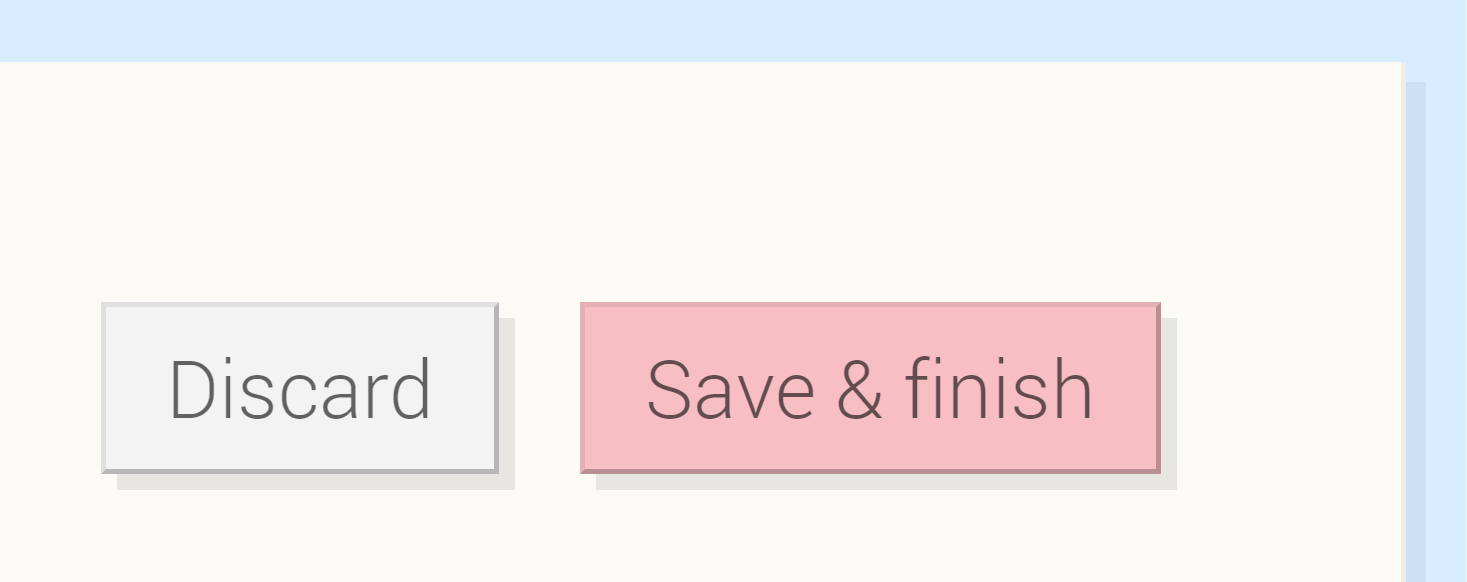
\includegraphics[width=\textwidth]{buttons.png}}
  \caption{Example of buttons}
  \label{fig:buttons_example}
\end{figure}

This is what Dieter Rams meant when he said that good design makes a product understandable. We can take the cornerstone element of every interface---a button---and use it as a kind of guinea pig. If we blindly followed the principles of flat design (which many do), the element's visual identity would quickly fall apart. But say we add a simple drop shadow---the metaphor then holds and so do the streamlined aesthetics. The point is that the button does not have to look exactly like a button to be recognized as one. Giving the user a cue is usually enough, his mind will do the rest and fill the gaps. The same applies for an input element---the user expects it to have at least a slight inset drop shadow and is confused when the element is not given one. This has been proven time and again by many usability studies.

\begin{figure}
  \setlength\fboxsep{0pt}
  \setlength\fboxrule{0.2pt}
  \fbox{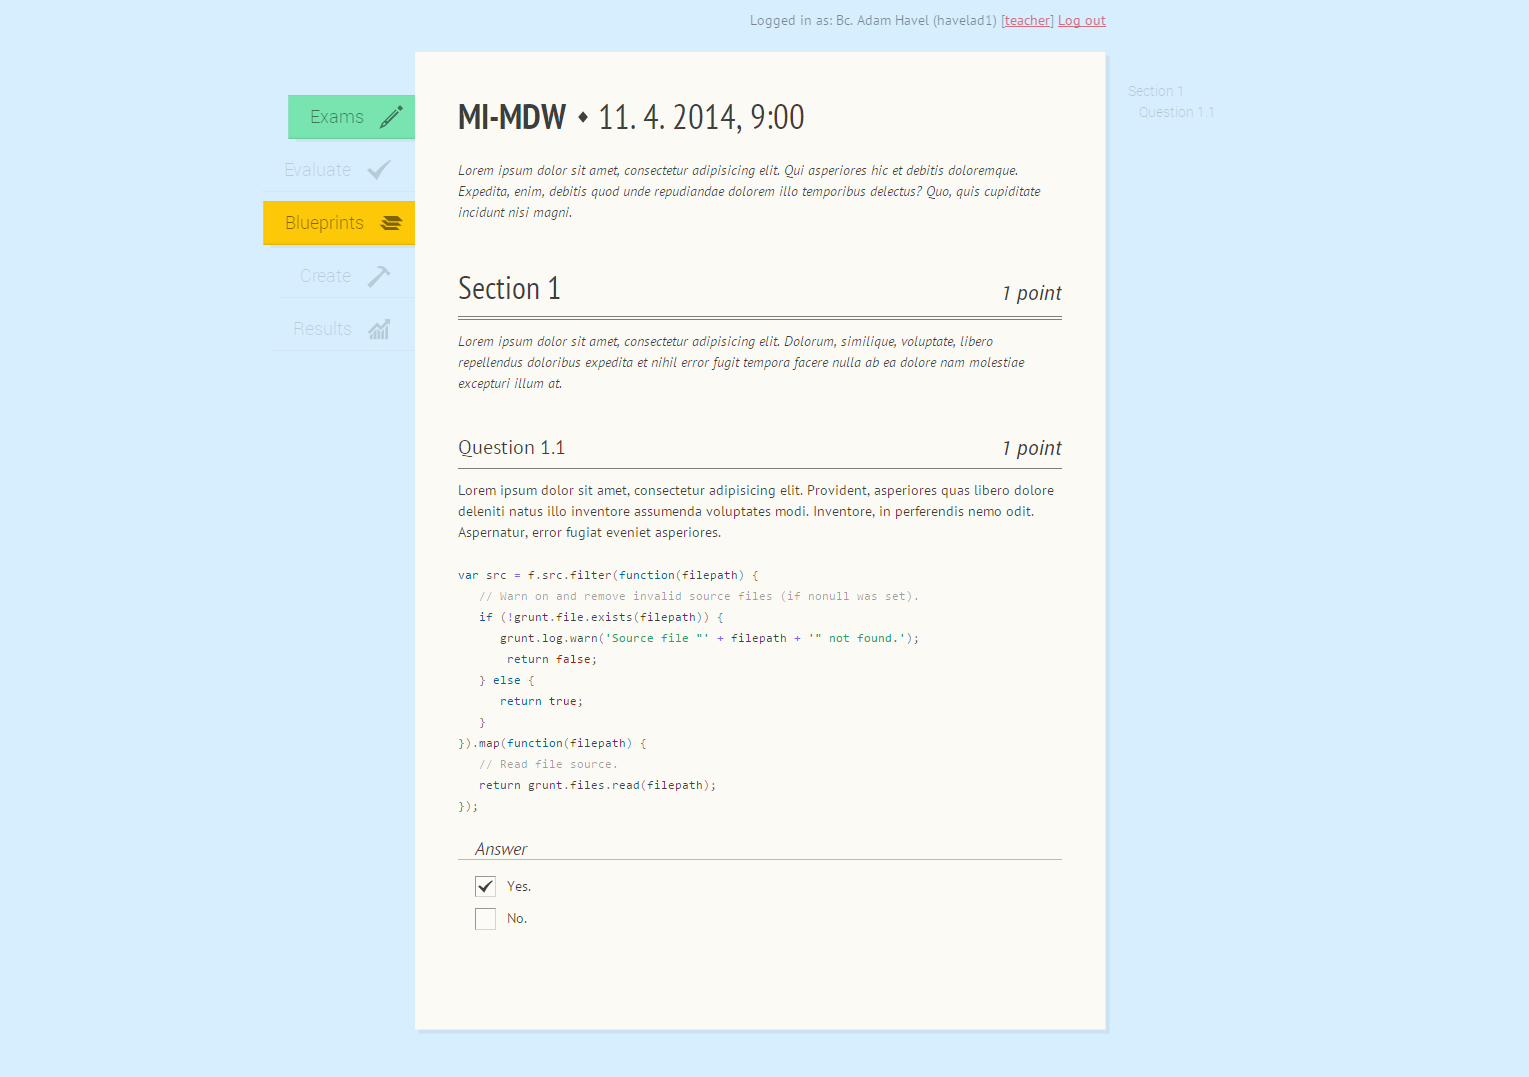
\includegraphics[width=\textwidth]{page.png}}
  \caption{Page layout}
  \label{fig:page_layout}
\end{figure}

It is because of these and many other reasons that the approach taken in designing the application user interface, while based on the principles of flat design in its focus on typography and color, is not shying away from some of the more reasonable aspects of skeuomorphism. Even though the design does rely heavily upon simple shapes and deliberate use of color, the most ostentatious attempt at emulating reality is immediately apparent when one takes a look at the page layout, as seen in the figure \ref{fig:page_layout}. The main content is presented in a form reminiscent of a sheet of paper. This is heightened by the use of color, a subtle drop shadow and the fact that when there is not enough content to stretch it further, the ``sheet'' holds a ratio of 1:1.414, the same as a real piece of paper. The reasoning behind this idea is to provide the users---especially the students---with something familiar. Novelties and surprises have their place in design, but one must choose wisely how and when to introduce them---confounding a student who is probably already struggling with his exam is hardly a good idea.

The side effect of this decision takes shape in the relatively small portion of the available viewport width being occupied by the main content, at least on displays designated for desktop use. This further strengthens the idea that the main content should always be in the spotlight. Any additional information that might not be essential but proves helpful is placed outside of this area---its opacity reduced unless in focus, in order not to distract the user. An example of such a component is the table of contents which apart from providing the document structure allows an user to tell his current position and to swiftly jump to a different part by way of anchor links.

The main navigation menu behaves similarly---translucent until the moment it is actually used. Only the active items are highlighted continually by taking on a likeness of bookmarks. Not just an aesthetic choice, this application of skeuomorphism is also meant as way to get across the idea that just like with a real book, there can be more than one bookmark at a time, each representing a shortcut to some point of interest.

    \subsubsection{Typography}

Notwithstanding the importance of aesthetic qualities, in the end, what matters the most is the actual content. In this case, the content is mostly textual, it is therefore necessary to make educated choices about the way the text is presented and structured. Such is the focus of the art of typography---arranging type in order to make the language it forms most appealing to reading and recognition. This involves the selection of typefaces, choosing the right font sizes and weights for each situation, adjusting the length and spacing of line, and much more.

\begin{figure}
  \setlength\fboxsep{0pt}
  \setlength\fboxrule{0.2pt}
  \fbox{
\includegraphics[width=\textwidth]{pt-sans.png}}
  \caption{Example of \textit{PT Sans} typeface}
  \label{fig:pt_sans}
\end{figure}

The first and probably most important decision is to pick the right typeface---one that hopefully reflects the qualities the product is trying to represent. In the case of this application, the choice came upon \textit{PT Sans}, a freely distributed font family that was released under the \textit{SIL Open Font License}. It was developed by a foundry called \textit{ParaType} under the sponsorship of the Russian government, as a way to provide a modern font that encompasses all characters contained within the many languages of Russian federation. It is a professional-grade typeface that combines traditional and conservative appearance with modern trends of humanistic sans-serif, and one that possesses an enhanced legibility. While choosing a serif font family would make more sense for longer passages of text, in this case the content is expected to consist of rather short snippets, sans-serif family therefore makes a better choice and matches nicely with the streamlined aesthetics of the application.

When combining different typefaces, it is necessary to pick font families that share similar x-height, which is---not very surprisingly---the height of the letter \textit{x} in a given font. If one does not feel adventurous, it is generally a good idea to choose typefaces from the same superfamily. The result is a set of fonts that, while belonging to different classes like sans and serif, have a similar appearance and properties, such as the aforementioned x-height. It is for these reasons that \textit{PT Sans Narrow} nicely complements the body text typeface while used in headings---the contrast such combination creates helps further define the document structure visually.

The same rationale has been used when selecting the \textit{PT Mono} typeface. It is a monospaced family which means the font's letters and characters each occupy the same amount of horizontal space. That makes it appropriate to use when displaying fragments of computer code or for numerical tabular data.

\begin{figure}
  \centering
  \setlength\fboxsep{0pt}
  \setlength\fboxrule{0.2pt}
  \fbox{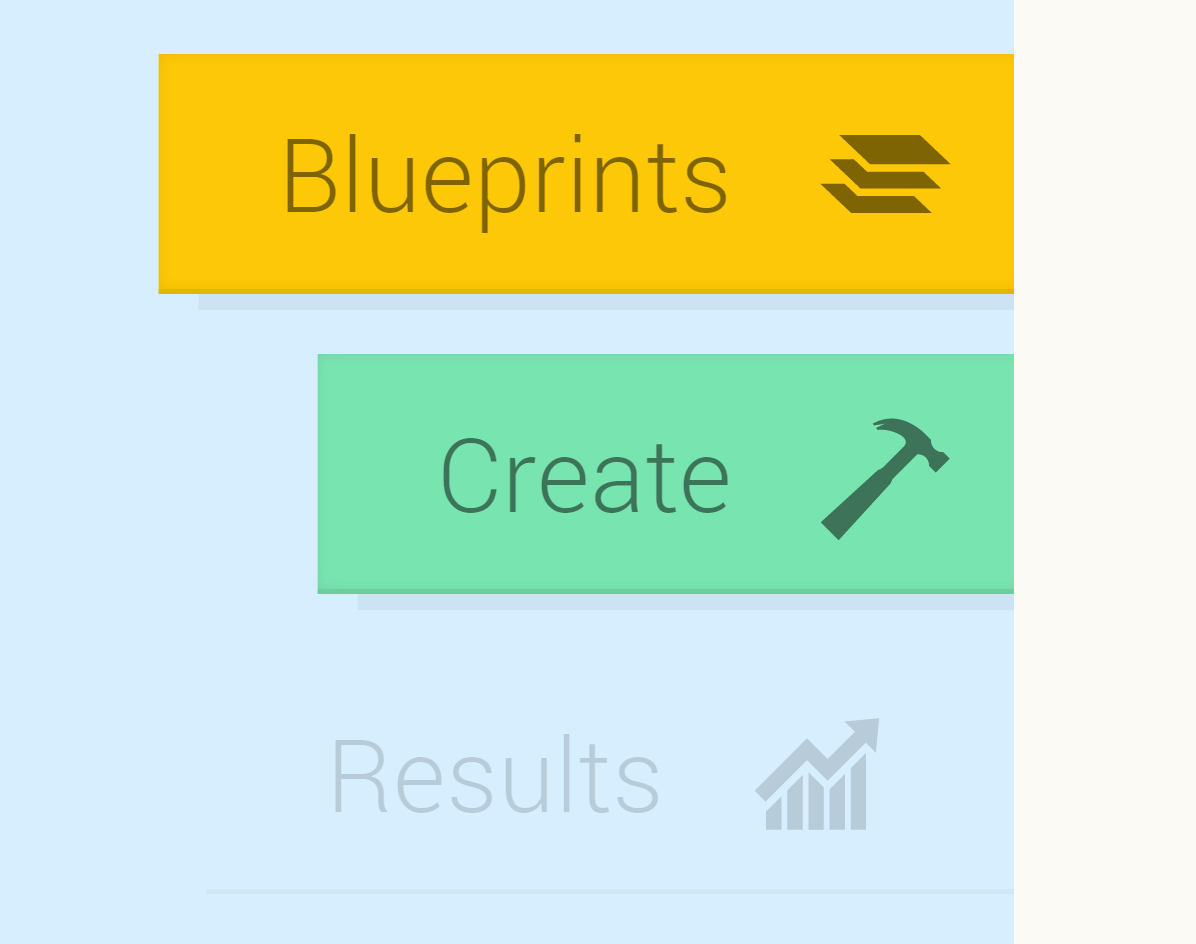
\includegraphics[width=0.66\textwidth]{roboto.png}}
  \caption{\textit{Roboto} typeface as used in the interface}
  \label{fig:roboto}
\end{figure}

Last on the list is \textit{Roboto}---a typeface developed by Google to serve as the default font family for the Android operating system. While often described as a ``Frankenstein among fonts'', because of the way it mixes different typographic styles, it is actually a good match for interface elements. It is therefore used in the navigation menu, and all the buttons and prompts.

Choosing the right font sizes for different contexts is usually next on the list and should not be done haphazardly---the whole layout of the page is (or should be) affected by the typographic decisions made, not the other way around. This is true for two reasons: first, the layout width should be set in such a way that any given line of text does not contain much more than around 70 characters---the amount which is believed to provide the best legibility. And second, all layout dimensions should be expressed in a relation to the base font size---this actually makes the first point trivial to achieve and is the raison d'être of the \code{em} unit. The base font size is however best left set at the default value of 1 \code{em}, which usually renders as a font size of 16 pixels. The user can then decide herself whether to enlarge or reduce the font size and changing thus proportionally the rest of the layout.

The moment we want to add different font sizes to our mix, we find ourselves at a crossroad. We can travel the path of arbitrary, conventional or easily divisible numbers, or we can use the so called modular scale. Making such scale is quite straightforward---a set of values is generated by choosing a number and a ratio, and multiplying or dividing the first with the other. In our case, the number is the base font size. As for the ratio, any proportion might do, but it is probably a good idea to pick one that is rooted in geometry, music, nature or history. Such ratios are culturally relevant and meaningful, and also tried and proven by centuries of use. More importantly, they tend to produce visually pleasing compositions.

The golden mean with its proportion of 1:1.618 is an obvious choice, but there are many others, equally useful. One of the simplest is the musical fifth with a ratio of 3:2. When put into our scale, it generates a value of 1.5 \code{em}---a good starting point for line spacing, which will be covered in a moment. Nonetheless, we might find that our set of values is too sparse and does not cover all needs. The remedy is often to create a double-stranded scale, one that is based not on one but two numbers. Like the first one, the second number should not be arbitrary---line length, which in our case equals 42 \code{em}, is usually a good choice.

\begin{figure}[h]
  \begin{lstlisting}
@mixin blank-lines($lines: 1, $direction: trailing, $type: margin) {
  $space: $lines * $leading;
  @if $direction == trailing {
    #{$type}-bottom: $space;
  } @else if $direction == leading {
    #{$type}-top: $space;
  } @else if $direction == both {
    #{$type}-top: $space;
    #{$type}-bottom: $space;
  }
}
  \end{lstlisting}
  \caption{Vertical rhythm in Sass mixin}
  \label{fig:vertical_rhythm_mixin}
\end{figure}

Another essential property is the already mentioned line spacing, also called leading. Using a value from the modular scale, it is set to be one and a half times of the font size. To further improve legibility, the leading of the body text is then chosen as the base for what is called the vertical rhythm---a principle of unifying the line heights of different elements so that each line, blank or not, can be expressed only as a multiple of this base. It is important to note that the base is no longer relative, i.e. expressed in \code{em}, but absolute. In the case of our body text with a font size of 16 pixels and line height set to 1.5 \code{em}, the base holds a value of 24 pixels. Multiples of this number are then used to define any line height, spacing or dimensions in the vertical direction. This is reflected in the style sheets, where except a few cases, every vertical \code{margin} or \code{padding} is expressed using the Sass mixin shown in the figure \ref{fig:vertical_rhythm_mixin}. The multipliers do not necessarily have to be integers but they should sum to a whole number. It is therefore allowed to have for example an element with margin of half the leading in both directions, since it adds up to one.

    \subsubsection{Colors}

The backdrop color has been chosen deliberately for its properties and effects on human mind. A light that is composed predominantly of the color blue has a direct and powerful influence on the secretion of melatonin, a hormone that regulates sleep patterns in mammals. So while it is generally a good idea to avoid blue light at night in order not to disturb one's sleep, the very same quality can be used during the day to effectively raise a person's alertness.

\begin{figure}[h]
  \begin{lstlisting}
$colors: (
  blue: #d7eeff,
  paper: #fbfaf5,
  yellow: #fdc807,
  red: #d1192b,
  green: #78e5b1,
  purple: #957bf8
);
  \end{lstlisting}
  \caption{Definition of colors in \textit{Sass}}
  \label{fig:sass_colors}
\end{figure}

While other colors might not have the same powerful properties, each of them holds some kind of meaning, which is more often than not defined a culture. It would be therefore unwise not to follow these leads and use the colors haphazardly. One simply has to know the product's target market and adjust accordingly to local traditions. Little details such as the fact that in the Japanese culture, the color white represents death may seem peculiar for us Westerners, but in the end do matter.

As already mentioned, the main content is filled with an off-white color expressed as a RGB hex triplet with a value of \code{\#fbfaf5}. Apart from trying to mimick the properties of a real paper, such color tends to be easier on eyes than pure white. The rest of the colors represent what is often called the brand of a product. They should be distinct enough so as to be immediately recognizable. In many cases, they are also employed as a kind of a visual cue to convey different meanings. These should be easier to grasp than for example a written prompt by itself---at least for those users that do not suffer from colorblindness. This approach is used for example in the navigation menu, as seen in the figure \ref{fig:menu}: a differently colored bookmark represents a different state of a given item. The yellow bookmark (\code{\#fdc807}) stands for the currently active page. The green one (\code{\#78e5b1}) hints at a work in progress. And when a bookmark turns red (\code{\#d1192b}), it is to draw attention to an urgent matter, for example exams that have yet to be evaluated.

\begin{figure}
  \setlength\fboxsep{0pt}
  \setlength\fboxrule{0.2pt}
  \fbox{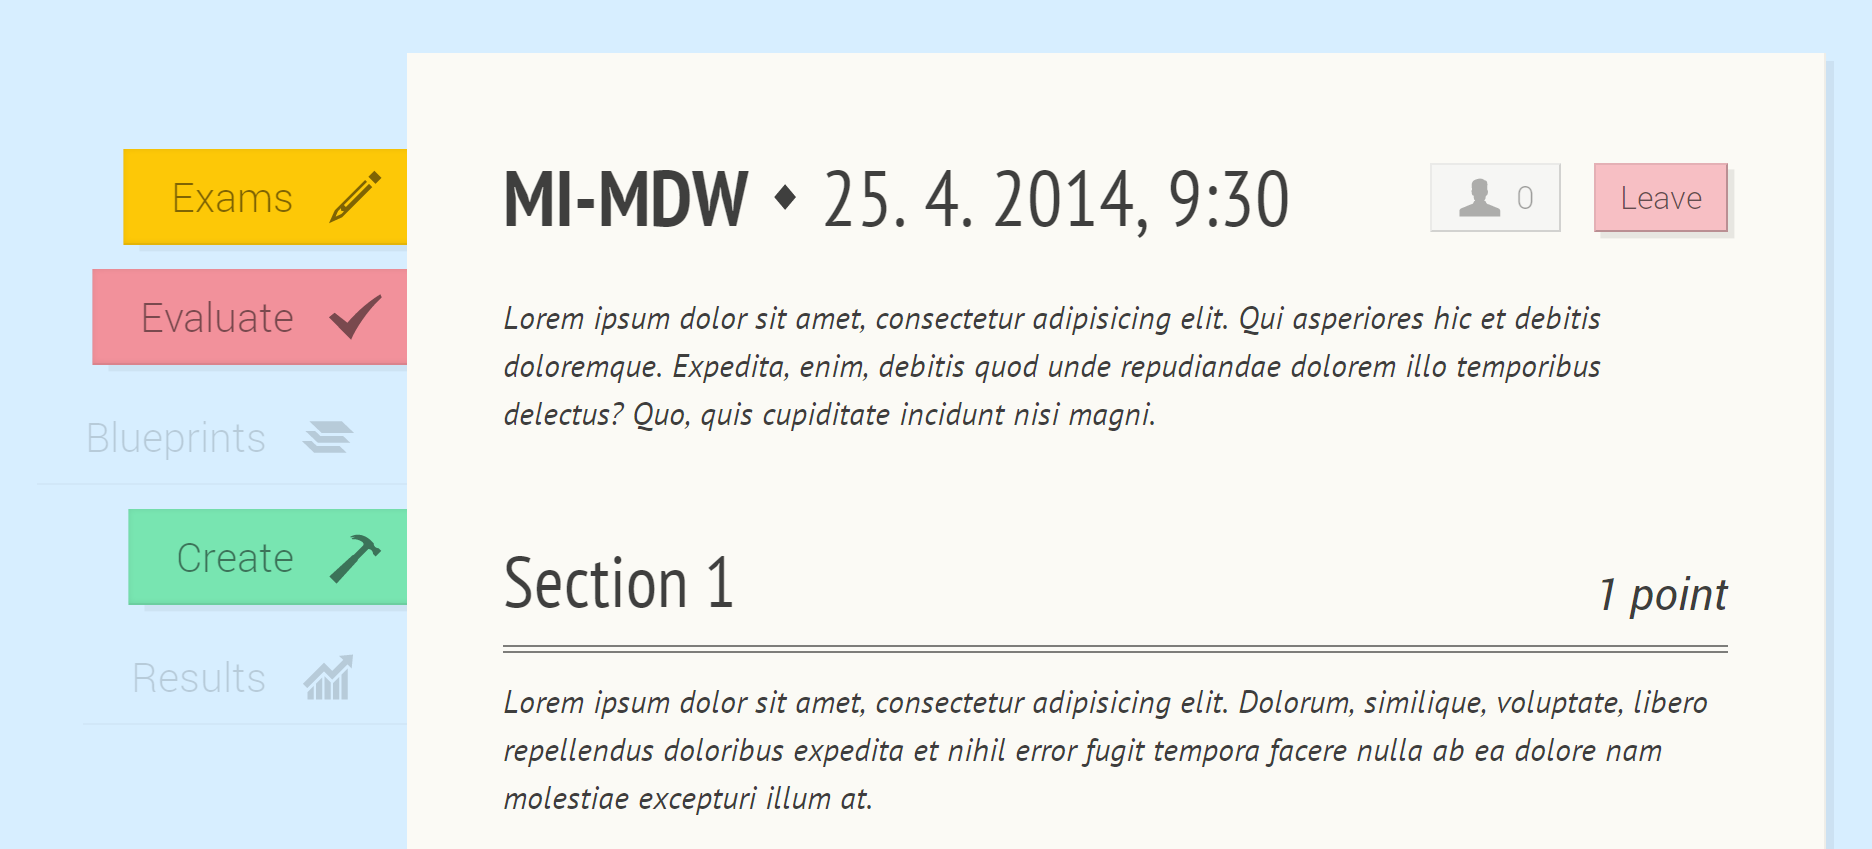
\includegraphics[width=\textwidth]{menu.png}}
  \caption{Use of colors in the menu}
  \label{fig:menu}
\end{figure}

To maintain a coherent visual identity, only the colors stated above and their variations are used throughout the application. The variations are created by means of two internal Sass functions: \code{ligthen()} and \code{darken()}. These functions take an original color as the first argument and an amount of change expressed in percentage as the second. The result is a color that is not different in hue from the original one---only the amount of white is augmented or reduced.

Anyhow, everything written about colors so far holds especially true for the so called modal windows. These are utilized heavily in the application and can be used as another example to further expand upon the argument for the importance of colors.

    \subsubsection{Modals}

A modal is a type of a child window that requires a user interaction in order to allow the user to return to the main window. They are used to draw attention to vital pieces of information or to display emergency states. And even though they are often criticized for breaking the user's workflow, they are irreplaceable in many situations. Most of their shortcomings can be remedied by using simple techniques such as darkening the background behind the window in order to focus the user's attention.

Another important aspect of modal windows is the fact that prompts tend to be either read wrong or not at all. It is therefore necessary to provide some countermeasures, in order to minimize the chance a user will do something he might regret later. There are several thing that can be done: first, as already stated before, it is important to create a consistent visual identity and adhere to it strictly. By using the color cues, a user is able to tell the general meaning behind a prompt, even before reading the message. And there is no need to go against the grain---an error message should be red and confirmation of success green. Yellow is meant to alert the user about a non-recoverable action he is about to make or in general any event that requires an immediate attention. Last but not least, purple holds the message that some kind of input---like submitting an image---is required in order to continue.

\begin{figure}
  \setlength\fboxsep{0pt}
  \setlength\fboxrule{0.2pt}
  \fbox{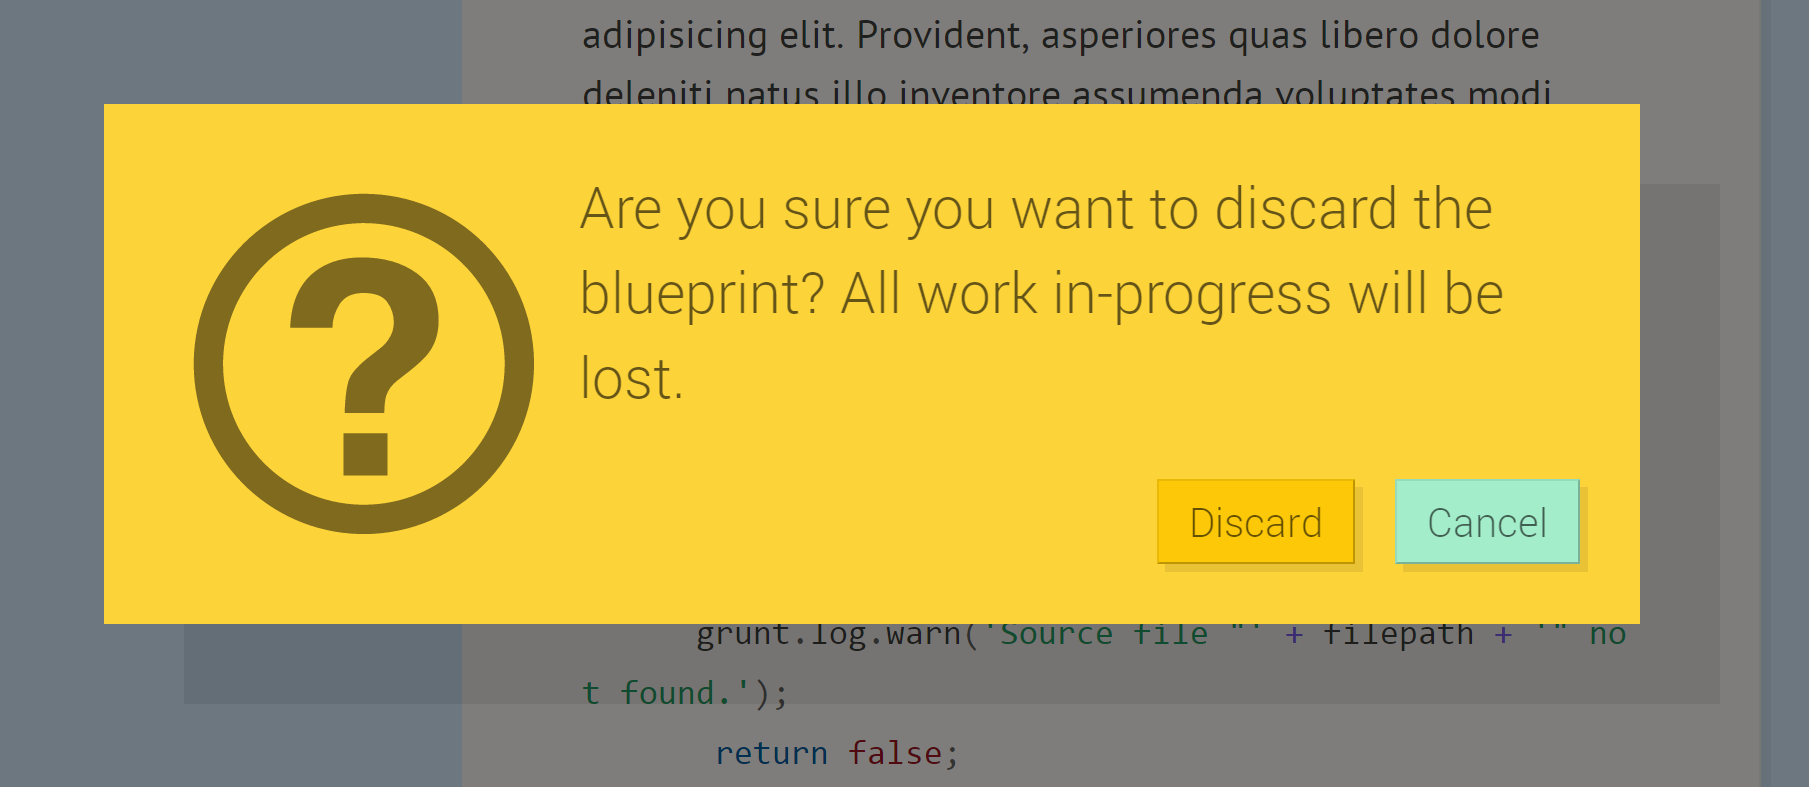
\includegraphics[width=\textwidth]{modal.png}}
  \caption{Modal window}
  \label{fig:modal}
\end{figure}

Furthermore, if possible, the user must be given a way to abort the action in question. This is usually accomplished by means of a cancel button. If present, it is also necessary to tell what is the primary action for given prompt. For example, when a modal warns the user he is about to delete something, the primary action is to cancel the removal. This is expressed in several ways. Visually, by emphasizing the cancel button and making the other, so called secondary action button less pronounced. Positionally, by placing the primary action button as the rightmost, which is the place the user is most likely going to click. And last, functionally, by binding it to the \code{enter} key.

    \subsubsection{Icons}

    ...

\begin{figure}[H]
  \setlength\fboxsep{0pt}
  \setlength\fboxrule{0.2pt}
  \fbox{
\includegraphics[width=\textwidth]{icons.png}}
  \caption{Example of icons}
  \label{fig:icons}
\end{figure}

  \subsection{Performance}

  ...

% Animations are a great way to enhance a user's experience with the application. They can help

\chapter{Processes}

  \section{Authentication}

No part of the system is accessible without authentication. Upon loading, the client makes a \code{GET} request to a resource defined at \code{/api/user} and appends a session identifier if a cookie is found. The server then tries to look up the identifier in MongoDB-backed session store. If successful, it checks whether the session has not expired---if that is not the case, it sends the client a JSON object containing information about the particular user. The information is obtained by deserializing the user identifier from the session and using it to fetch relevant data from the database. The client application then fills its \code{User} service with the received object and the user is onward recognized as authenticated.

    \subsection{Logging in}

In the opposite case---either no session was found or it has already expired---the server responds with a 401 status code which forces the client to show the user to a login form. After filling in the form, the client makes a new request to the \code{api/user} resource, this time using the \code{POST} method, sending along user credentials. These credentials are then checked against a faculty LDAP server running at \code{ldap.fit.cvut.cz} using a secure connection. If user's identity is verified, the LDAP server responds with basic information about the user. Back at the application server, the database is queried for additional data using the user identifier. It either finds a relevant entry or not. In the former case, the entry is updated with a new timestamp, representing the last login time, and the server sends it to the client as a JSON object, the same as before. If the latter is the case, it means that the user is logging in for the first time.

\begin{figure}
  \setlength\fboxsep{0pt}
  \setlength\fboxrule{0.2pt}
  \fbox{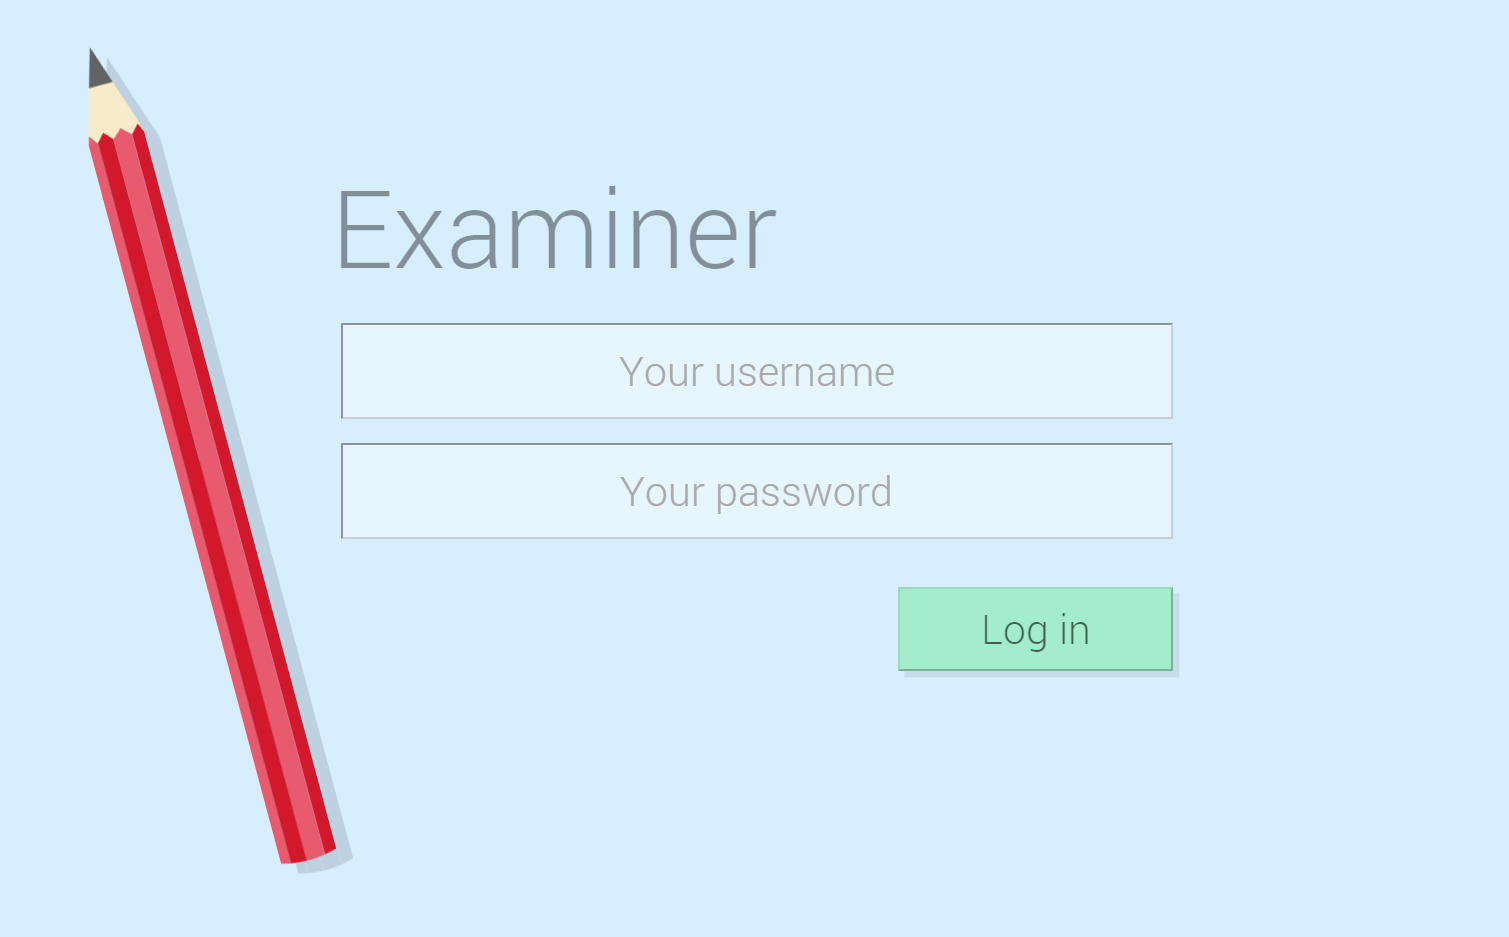
\includegraphics[width=\textwidth]{test.png}}
  \caption{Login form}
  \label{fig:login_form}
\end{figure}

A new instance of \code{User} model is then created and filled with the available data. What remains unknown is the user's role---that is, if he or she is a student or a teacher. That information can be obtained by making a request to \textit{KOSapi}, a faculty service that provides a REST API over the university information system \textit{KOS}. To find out the role of a person with a given user identifier we can utilize the resource \code{/people/\{uid\}}. With that issue resolved, we can continue by looking up all courses the user either studies or teaches by using the resources \code{/students/\{uid\}/enrolledCourses} and \code{/teachers/\{uid\}/courses}, respectively. It is worth noting that \textit{KOSapi} returns the data formatted as XML, which means the server has to transform it into a JSON object, for which it uses an external library called \textit{x2js}. After obtaining all the necessary data, the new user can finally be saved in the database and sent to the client.

But since both the role and the subjects of a user can change, the server has to periodically request the current states of the aforementioned resources and make necessary changes in the application database. This is one of the reasons the last login time is saved in the \code{User} model---using this information, the server makes sure not to ask for new data more than once a day. And since the majority of these changes occur at the start of a semester, long before any exam takes place, it should be frequent enough for most cases.

    \subsection{Client-side verification}

When the client receives the authentication data and stores it in the appropriate service, the user can start to use the application with the scope assigned to his role. If for some reason the \code{User} service gets unset again, the user is shown a login form and any navigation elsewhere is disabled until he successfully logs in. In this manner, the authentication is verified only via the client-side service which might not be up to date with the server. This is sufficient for some operations and serves to mitigate any latency that would arise from communication between the client and the server.

If the user logs out, the \code{User} service is emptied and the client sends a \code{DELETE} request to the \code{/api/user} resource which prompts the server to discard the session. Nonetheless, the client session might also be terminated at the server end, either by force or because it has expired. It is therefore necessary that the client recognizes this situation and acts accordingly. This is ensured by using a HTTP interception service that monitors every response the client receives from the server when it tries to reach a resource. Whenever a 401 status code shows up, it means the session has been ended and the user has to authenticate again if he wishes to continue.

\begin{figure}[h]
  \begin{lstlisting}[language=JavaScript]
app.factory('AuthInterceptor', function($q, $injector, Modal) {

  return {
    'response': function(response) {
      if (response.status === 401 && $injector.get('User').data) {
        Modal.open('alert', 'Your session has been ended. You will have to authenticate.', null, 'Log in');
        $injector.get('User').logout();
        return $q.reject(response);
      } else {
        return response || $q.when(response);
      }
    }
  };

}).config(function($httpProvider) {
  $httpProvider.interceptors.push('AuthInterceptor');
});
  \end{lstlisting}
  \caption{HTTP Interceptor}
  \label{fig:http_interceptor}
\end{figure}

The HTTP interceptor can be seen in the figure \ref{fig:http_interceptor}. It requires the \code{User} service so that it can tell whether a user is present and to log him out if necessary. In any other type of component, the \code{User} service would be injected normally, but that is unfortunately not possible in this scenario. The problem arises from the fact that injecting a service into another component makes it dependent on that service. And since the \code{User} service is already dependent on \code{\$http} and applying the interceptor essentially modifies the instance of the very same \code{\$http}, making \code{\$http} dependent on the \code{User} service through the interceptor would create what is called a circular dependence. That can be remedied by using the built-in \code{\$injector} service which is able to get hold of another service reference without creating a dependence.

Something similar to the 401-filled responses also occurs when a user is not authorized to view a selected resource. This applies for example in the case when a user with the role of a student requests a different student's results. When such a thing happens, the server responds with a status code 403. Nevertheless, such request is never made on behalf of the client application and can only occur when the user tries to reach the server resource directly, via the provided API. That is why we do not have to handle this problem on the client side.

  \section{Blueprints}

A blueprint represent what in real life would be the original copy of a written test. In the application, blueprints can be created, viewed and modified until the day of the exam. Quite obviously, all of these operations are allowed only for users that hold the role of a teacher. And even those can manage only the blueprints that belong to the courses they teach.

    \subsection{Resources}

The blueprints are exposed as two resources, each of them designed for different use. The first one represents a collection of blueprints and is accessible via \code{/api/blueprints}. It supports optional query parameters for filtering by subject, date and language. When no subject is specified, the result is automatically filtered using the list of subjects contained in the \code{User} service. If, on the other hand, a subject is given, it is tested against the same list and if no match is found, the server responds with a 403 code. Otherwise, the query is passed along.

In the end, the resource returns a collection of all the blueprints in the database that satisfy the inherent or supplied conditions. Anyhow, since the resource is used only for listings on the client side, it is unreasonable to request the actual content of the blueprints. Sending just the basic information will suffice and anything more than that would be a waste of bandwidth. To trim the response, the client can use the optional parameter \code{fields}. It is available to all the resources the API provides and when given, it prompts the server to return only the specified fields.

The other resource is used for operations dealing with a particular blueprint and can be found at URI \code{api/blueprint/\{subject\}/\{date\}/\{language\}}. Note that the variables are not optional and must be validated before any further processing, otherwise the server returns an error. The subject must be a valid subject code---starting with either \code{MI} or \code{BI} depending on the level of the subject, followed by a hyphen and ending with three word characters. The date must represent a string formatted as \code{YYYY-MM-DDThh:mm}, for example \code{2014-04-25T07:51}, and the language is validated against the standard \textit{ISO 639-1} which allows only codes like \code{en} or \code{cs}.

The combination of these three variables is the only unique identifier of a blueprint in the application. There is a different type of key we might have used, which is the entry identifier assigned to every exam term in \textit{KOS}, but because of the fact that an exam can be taken in different languages at once, it would not suffice. Even though such case is not very probable, it could still happen, and there is no reason for the application not to be as flexible as possible. It also helps retain a certain human-friendliness, as opposed to having to query the server API using generated identifiers.

    \subsection{Viewing blueprints}

To view the blueprints, which only teachers are allowed to, the user must navigate to the state \code{Blueprints} which results in URL \code{/blueprints}. The items depicted are organized in stacks which reflect the logical distribution of blueprints among subjects. If only one subject is available, the user is presented directly with individual blueprints. Clear graphical distinction is made between what is considered stack and what is an individual ``sheet'' so that the user quickly recognizes which is which. Apart from using the browser history, the user can navigate the blueprints using a breadcrumbs navigation. This is possibly excessive in this case but makes more sense in different listings, for example when viewing exams where the structure depth can reach four levels. Also important is the fact that the current level is shared among all listings, which should help with the workflow. Anyhow, the listing is empty so far because we have yet to create our first blueprint.

    \subsection{New blueprint}

To create a new blueprint, the user must enter the state \code{NewBlueprint} which is reflected in the URL as \code{/new}. She is then shown a listing similar to the one before, only this time with exam terms instead of blueprints. Terms are the particular dates on which an exam takes place---we can get those by reaching the \textit{KOSapi} resource \code{/courses/\{subject\}/exams}, using each of the user's subjects for the variable, one after another. The client actually asks the application server resource \code{api/examterms} which delegates the request to the aforementioned endpoint. The result is then stripped of any term that is already fully occupied with blueprints in the database.

When a term is picked, the user is presented with a modal window requesting the language of the exam. This step is skipped if no choice is available or only one language is left. Afterwards, the user can finally proceed with the new blueprint.

The blueprint is initialized with one empty section that cannot be deleted and which is given a default name, unless changed. By using the controls, one can create another sections, move them up or down, or delete them along with their contents---as long as there is at least one section left. If needed, the user can also write a short introductory paragraph for the whole exam or for each of the sections.

When a new question is added to a section, the user must fill it up with content, which is divided into two parts---the body of the question and the answer. Both consist of a set of content blocks of different types that can be moved up or down the body and removed individually. This is achieved through controls pictured in the figure \ref{fig:new_blueprint}. When deleting a block---be it a chunk, a question or a whole section---the user is prompted if she really wishes to continue. If empty, the block is removed automatically.

\begin{figure}
  \setlength\fboxsep{0pt}
  \setlength\fboxrule{0.2pt}
  \fbox{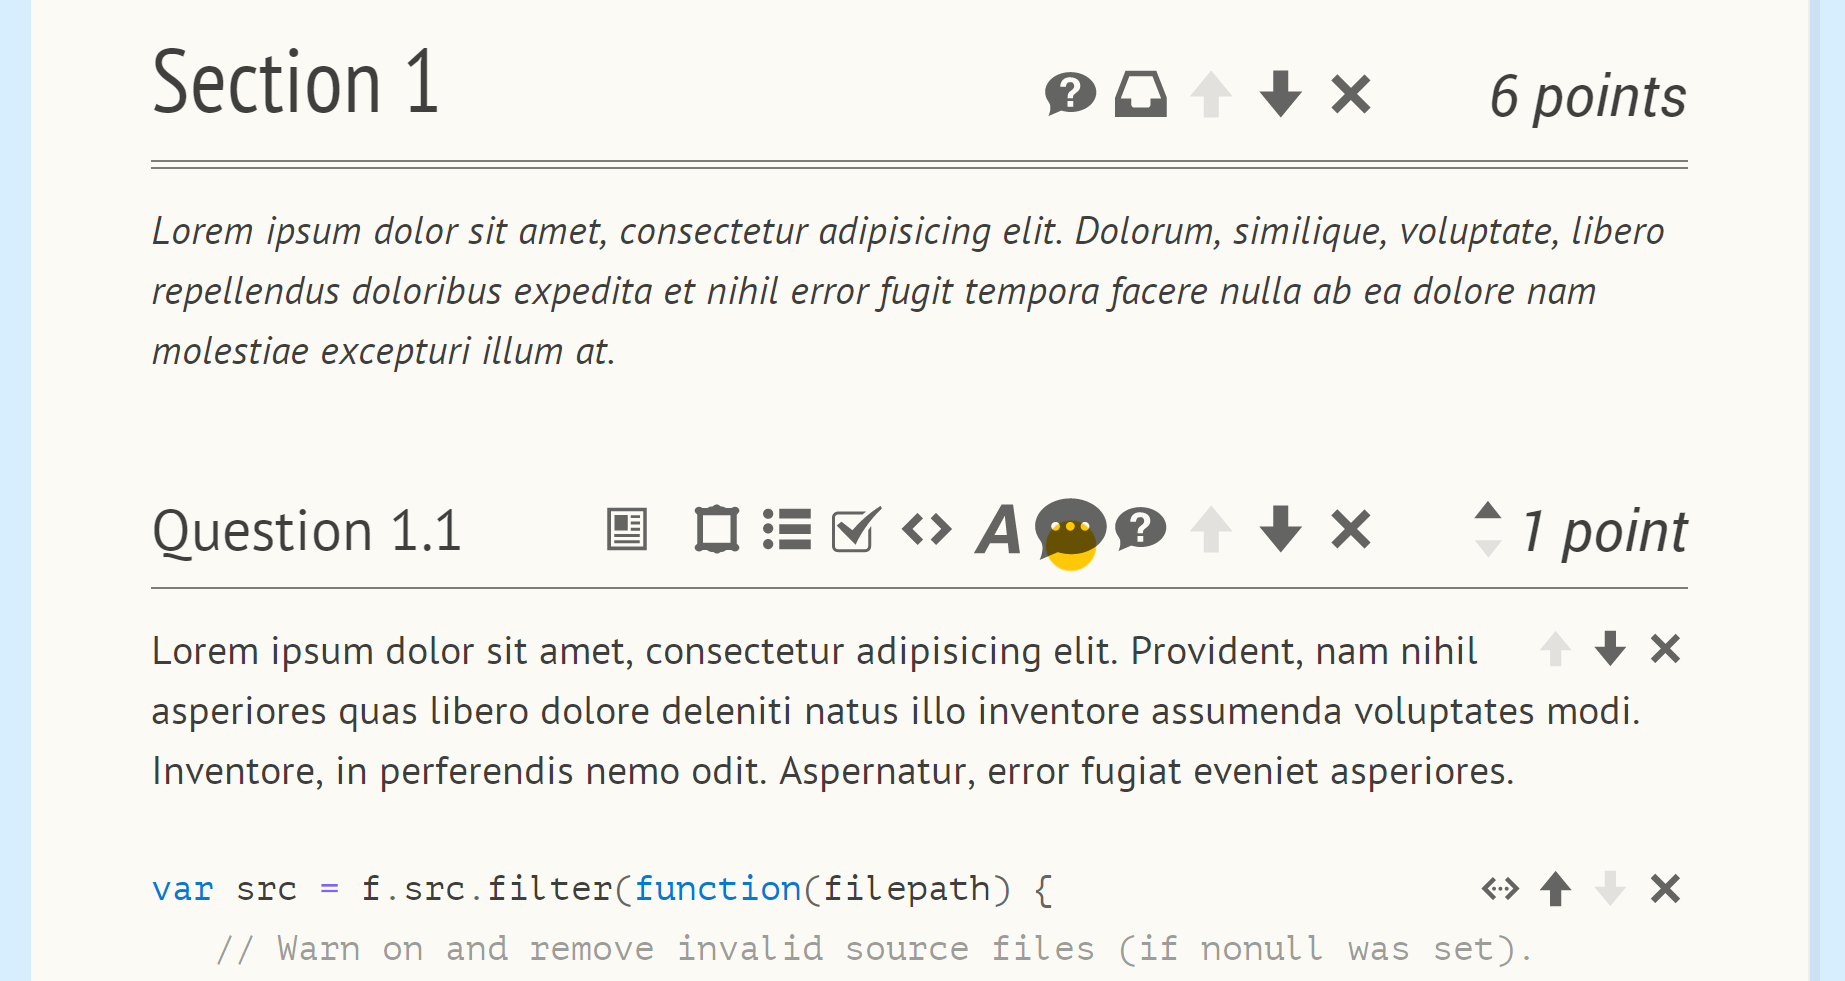
\includegraphics[width=\textwidth]{new-blueprint.png}}
  \caption{Creating a blueprint}
  \label{fig:new_blueprint}
\end{figure}

The types of content that can be added to the question's body and answer are a little different, depending on the target. It would for example make no sense to add an external image to the answer or a list of options into the body. Otherwise, the choices are the same---the user can add a paragraph of text, a snippet of code, a list, or a canvas. In the case of a snippet, the user has to pick a programming language, which can be changed anytime later. If adding an external image, a link must be provided which is then validated by creating a JavaScript \code{Image} object having the URL for its source. If the object throws an error, it means the link is either broken or that the resource is not a valid image. Since downloading the image might take some time, it is necessary that the function---seen in the figure \ref{fig:image_validation}---returns a promise object, constructed via the service \code{\$q}. Either way, the \code{Image} object is then destroyed, even if having passed the test---the image is already in the cache so there is no reason to keep it in the memory.

\begin{figure}[h]
  \begin{lstlisting}[language=JavaScript]
function isImage(src) {
  var deferred = $q.defer(),
      image = new Image();

  image.addEventListener('error', function() {
    deferred.resolve(false);
  });
  image.addEventListener('load', function() {
    deferred.resolve(true);
  });

  image.src = src;
  image = null;

  return deferred.promise;
}
  \end{lstlisting}
  \caption{Validating an image}
  \label{fig:image_validation}
\end{figure}

After creating the answer which usually consists of just one chunk of content, the user can fill it with a solution. This will help in the future evaluation. It is also possible to create a hint that takes a form of a pre-filled answer. When added, the hint has the same content as the solution. It is therefore necessary to delete anything the user creating the blueprint does not wish the students to see.

When finished, the user can save the blueprint in the database. First, the blueprint is checked as to whether it meets the necessary conditions---it must contain at least one question and no question can be empty or without a defined answer. The blueprint is then saved into \code{localStorage}, in case something goes wrong. Only when successfully backed up, the process continues by converting chunks of the canvas type into SVG strings, and stripping snippets of any HTML---at least the kind that has been used for highlighting the code.

The blueprint is then finally passed to the server-side resource by means of \code{POST}. Before storing in the database, any SVG string inside the blueprint is optimized using the \code{SVGO} library---doing this can greatly reduce the size of the string. A blueprint stored in this way can later be modified, but only if it has not yet been used for an exam.

    \subsubsection{Cloning blueprint}

While creating a blueprint, the user can browse the old blueprints via the \code{Blueprints} state like she would normally do. The difference is that she is now given an option to copy an already defined question into the new blueprint. It is also possible to copy an entire blueprint---any work already done will be replaced by an exact copy of the given blueprint, except the main identifiers like subject or date, which remain intact.

\begin{figure}[h]
  \begin{lstlisting}[language=JavaScript]
NewBlueprint.data.sections = JSON.parse(JSON.stringify($scope.blueprint.sections, function stripJunk(key, value) {
  if (/^[\$_]/.test(key)) {
    return undefined;
  }
  return value;
}));
  \end{lstlisting}
  \caption{Cloning a blueprint}
  \label{fig:cloning_blueprint}
\end{figure}

One of the easiest and fastest way to clone an object in JavaScript is to use the complementary functions \code{JSON.stringify()} and \code{JSON.parse()} in sequence. However, when cloning the blueprint, an extra caution must be taken not to copy properties such as \code{\_id}, created while previously saving the object in the database. Otherwise, the new blueprint could not be stored. This can be done by employing the optional second parameter of \code{JSON.stringify()} which expects a function. The function can be used to reject a property depending on its name or value, and can be seen in the figure \ref{fig:cloning_blueprint}.

  \section{Exams}

When referring to exams, it is important to note the difference between an exam term, as described before, and an exam in the sense of a particular student's exam.

    \subsection{Viewing exams}

When viewing the exams via the state \code{Exams} located at \code{/exams}, the individual items represent available exam terms. The definition of what available means differs depending on the role of a user---a teacher sees any pending exam term that is listed in \textit{KOS} and belongs to one of his subject. A student, on the other hand, is shown only the terms for which he applied in advance. Both lists can be obtained by using the already mentioned \code{api/examterms} resource.

    \subsection{Ongoing exams}

By selecting an exam term, the client creates a new WebSocket connection which will be used by the server to handle communication among different users at the same exam. While this holds true for both students and teachers, what follows after is largely dependent on the user's role, it will therefore be explained separately.

      \subsubsection{Watching over exams}

A teacher can see the exam---exactly as it will be shown to students---right from the beginning. Furthermore, he is given the option to temporarily show the solution to any question. Until the moment the first student appears, he can also leave and therefore abort the exam. Whenever a student enters the exam, the teacher is sent a message containing all the necessary information. Since there can be more than one teacher watching over an exam, the message is actually sent to all of them. If any of these arrives late and identifies himself as a teacher, he is provided a list of students that are already present at the exam.

After making sure that all students at the exam are also physically present in the same room---which can be verified by the application itself by checking IP addresses of all the users and ensuring they all share the same subnetwork mask---any of the teachers can ``hand out'' the tests. That entails setting the exam duration. If necessary, the timer can be later adjusted. Nonetheless, when the time runs out, the exam is finished and all users are forced to leave.
Teachers may also decide to collect the tests early, which has the same results.

      \subsubsection{Taking exams}

A student can enter the exam only when a teacher is already present. Before allowed further he is also shown a modal citing a passage from the Ethical codex of CTU in Prague which he has to acknowledge in order to continue. While seemingly a superfluous formality, the reasoning behind this step is actually quite complex. The idea is based on the research by Dan Ariely, professor of psychology and behavioral economics, who led a series of experiments on cheating.

For a long time it was thought that people cheated by employing a rational cost/benefit analysis. When tempted to engage in an unethical behavior, they would weigh the chances of getting caught and the resulting punishment against the possible reward, and then act accordingly. However, experiments by Dr. Ariely and others have shown that far from being a deliberate, rational choice, dishonesty often results from psychological and environmental factors that people typically are not even aware of.

\begin{figure}
  \setlength\fboxsep{0pt}
  \setlength\fboxrule{0.2pt}
  \fbox{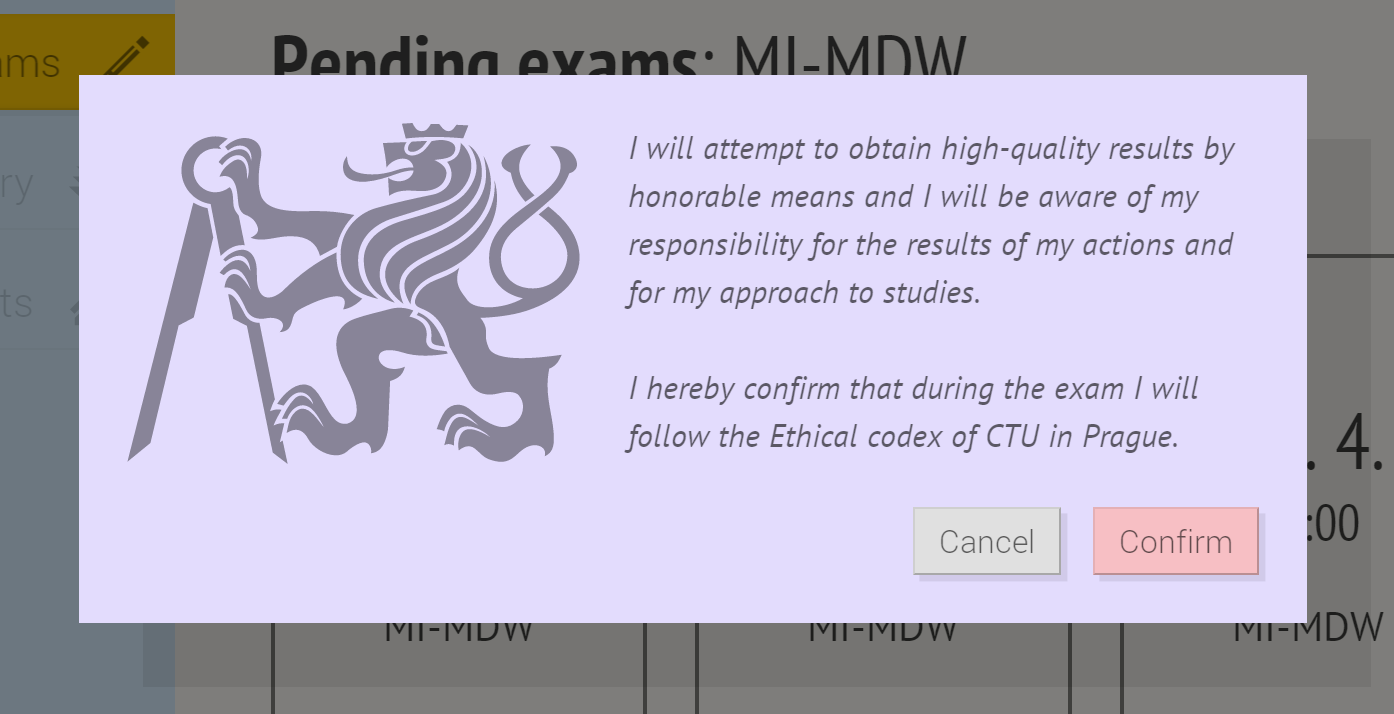
\includegraphics[width=\textwidth]{ethical-codex.png}}
  \caption{Acknowledging the Ethical codex}
  \label{fig:ethical-codex}
\end{figure}

Ariely discovered this truth by constructing a set of experiments with group of students from the universities of MIT and Yale. The participants sat in a classroom-like setting and were given tests. To create an incentive, the students were also given a certain amount of money for every right answer. Each of the experiments was then held under different conditions---making the cheating either less or more possible. In the end, Ariely found that given the chance, lots of people cheated---even if just a little.

Ariely then conducted another experiment, only this time the students had to sign a statement that said: ``I understand that this experiment falls under the guidelines of the MIT/Yale honor code.'' The act of signing resulted in zero cheating, and this was true even though neither university actually has an honor code. As Ariely concluded from this line of his research, ``recalling moral standards at the time of temptation can work wonders to decrease dishonest behavior and potentially prevent it altogether.'' Reminding the student that there is such a thing as the Ethical codex will hopefully have a similar effect.

Upon entering the exam, the menu is hidden and every attempt at navigating elsewhere manually is forbidden. The student is not allowed to see the test until a teacher ``hands it out.'' When that happens, he is notified and told the time at which the exam ends. During the exam, the time left is visible in the form of a timer which calculates the value internally using the function \code{setInterval()}. Even though the single-threaded nature of JavaScript and the inherent imprecision of its timing functions does not allow us to utilize the function directly to count the time, it can be used to periodically compare the current timestamp against the time of the exam's start. That way, we can obtain a fairly precise data that can be displayed to the user. To confuse the timer, the user might try to change the system time of his computer, which would work---but only locally. The end of the exam is determined exclusively by the timer running on the server. When that runs out, every user is forced to leave despite the time shown on their local timers.

The moment the user starts to answer the questions, his responses are sent to the resource \code{api/exam/\{subject\}/\{date\}/\{language\}/\{uid\}} using the \code{PUT} method and backed up in the database. This process is handled by a set of event listeners that are attached to each of the questions and which react to input. In order not to flood the server, the so called debouncing is employed. It refers to a technique where a function is run only if a defined amount of time has passed since the last time it has been called.

A student can also ``hand in'' the test early, if he wishes to. The data is then prepared in the same way as in the process of creating a blueprint---canvases are transformed into SVG strings and snippets are stripped of any HTML. The result is then sent to the server and if successfully stored, the student is notified and redirected to the homepage, his navigation rights returned.

      \subsubsection{Prevention of cheating}

While hopefully not an omnipresent factor, cheating still has to be taken into account---there are several ways the student could take advantage of the fact that the exam is taken on computer, even in the case of restricted network access. In order to prevent---and possibly discourage---the student from any attempt at cheating, two different techniques are used.

The first one employs the \code{blur} event of the \code{window} object which is fired whenever a page loses focus---either because the tabs in the browser were switched or because the browser itself lost focus in favor of some other application. When that happens, all teachers at the exam receives a notification pointing at the incriminated student.

Nonetheless, if applied by itself, a resourceful student still might think of a way to evade this countermeasure. If he prepared a file with notes in advance and resized the browser window so that the file can be seen---without having to switch between the applications---the first technique alone cannot stop him.

To handle the aforementioned situation, a different technique is utilized. Whenever a student tries to resize the browser, an event is fired. The client application on the student's computer then calculates the usage of the screen which is achieved by dividing the available viewport of the computer (\code{window.screen.availWidth} × \code{window.screen.availHeight}) by the dimensions of the browser window (\code{window.outerWidth} × \code{window.outerHeight}). If under 100 \%, teachers are notified and shown a modal which informs them of the student in question and the percentage of screen covered by the browser. The same calculation also commences automatically at an exam start, in case a student resizes the screen in advance.



\begin{figure}
  \setlength\fboxsep{0pt}
  \setlength\fboxrule{0.2pt}
  \fbox{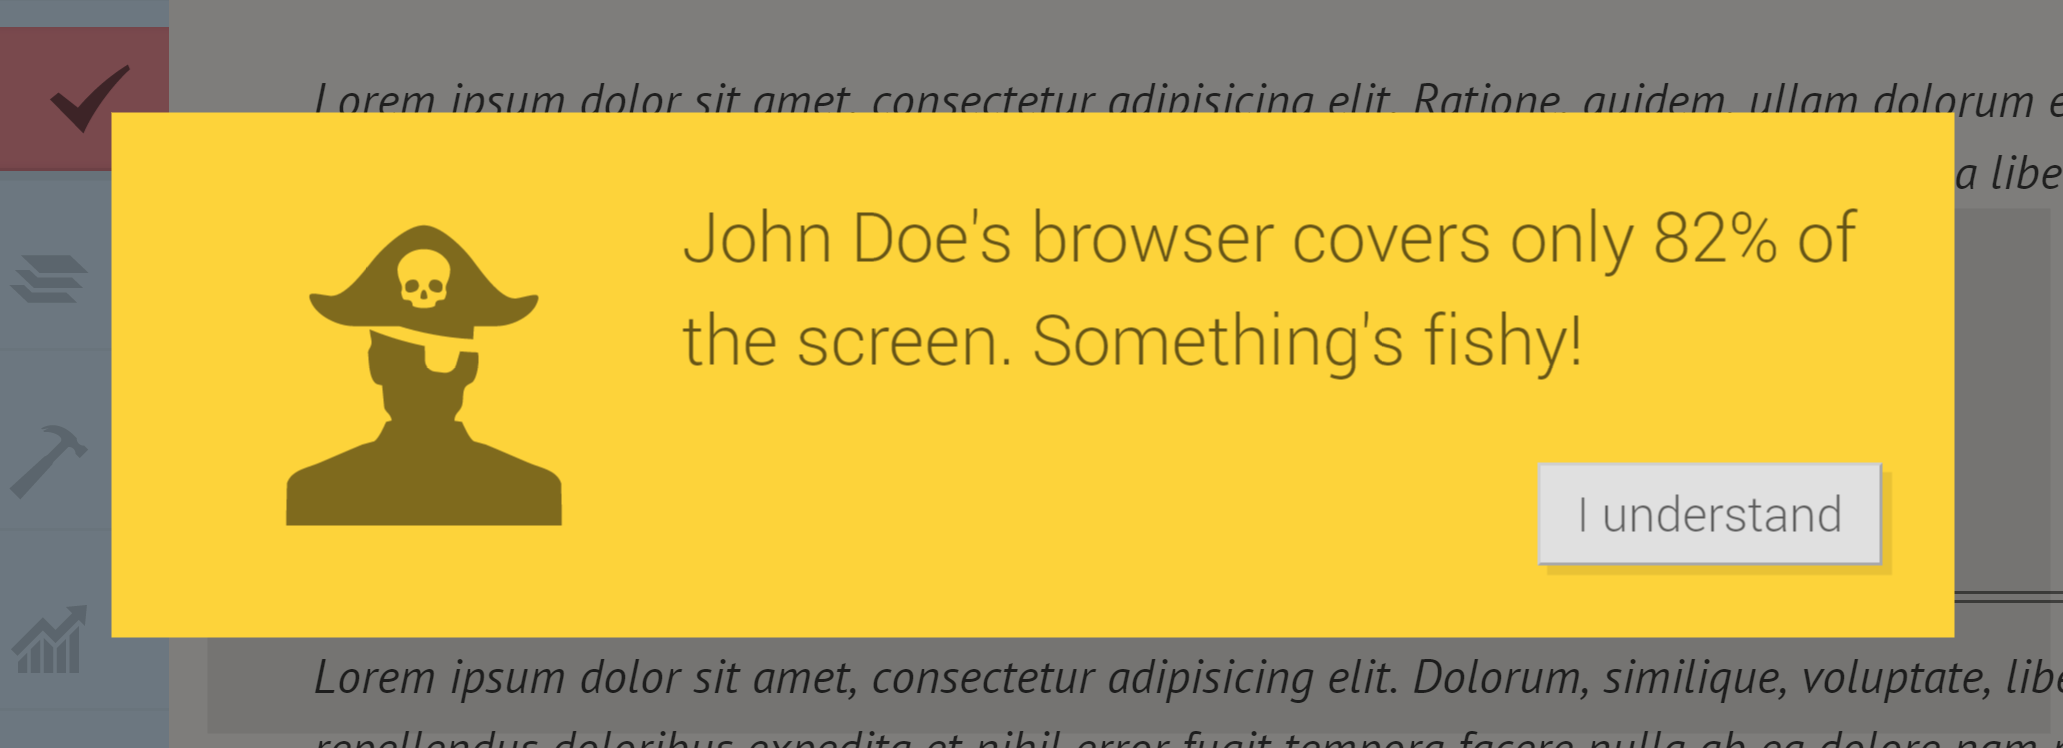
\includegraphics[width=\textwidth]{cheating.png}}
  \caption{Notification of window resize}
  \label{fig:cheating}
\end{figure}

    \subsection{Evaluation}

    ...

\begin{figure}[H]
  \setlength\fboxsep{0pt}
  \setlength\fboxrule{0.2pt}
  \fbox{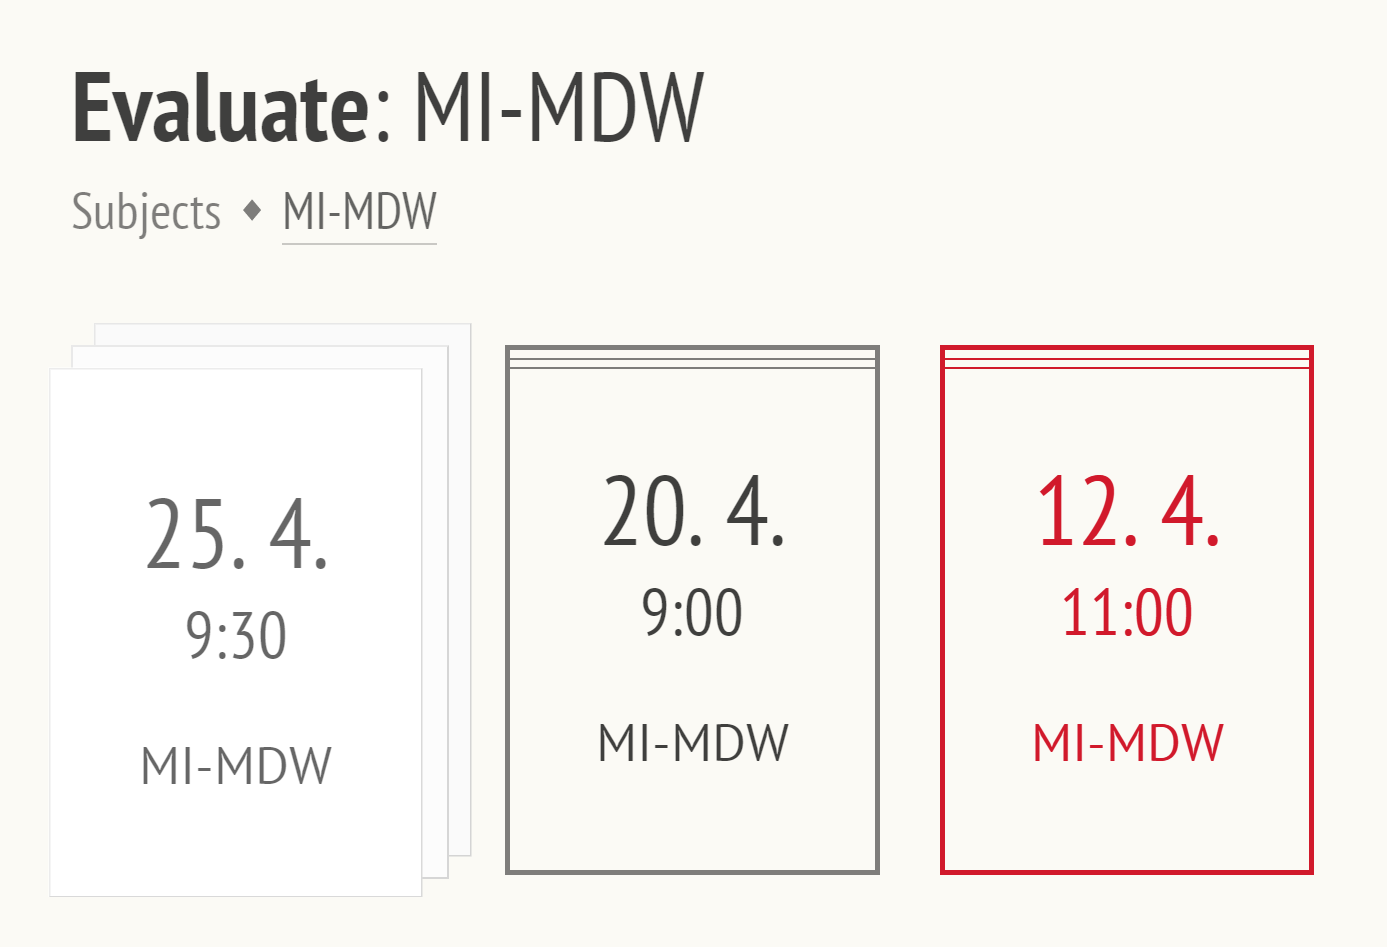
\includegraphics[width=\textwidth]{listing.png}}
  \caption{Example of listing}
  \label{fig:listing}
\end{figure}

\setsecnumdepth{part}
\chapter{Conclusion}


\bibliographystyle{iso690}
\bibliography{mybibliographyfile}

\setsecnumdepth{all}
\appendix

\chapter{Acronyms}

\begin{description}
  \item[API] Application Programming Interface
  \item[CSS] Cascading Style Sheets
  \item[DOM] Document Object Model
  \item[DRY] Don't Repeat Yourself
  \item[HTML] Hypertext Markup Language
  \item[HTTP] Hypertext Transfer Protocol
  \item[JSON] JavaScript Object notation
  \item[LDAP] Lightweight Directory Access Protocol
  \item[REST] Representational State Transfer
  \item[SVG] Scalable Vector Graphics
  \item[XML] Extensible Markup Language
\end{description}


\chapter{Contents of enclosed CD}

\begin{figure}
   \dirtree{%
      .1 readme.txt\DTcomment{the file with CD contents description}.
      .1 exe\DTcomment{the directory with executables}.
      .1 src\DTcomment{the directory of source codes}.
      .2 wbdcm\DTcomment{implementation sources}.
      .2 thesis\DTcomment{the directory of \LaTeX{} source codes of the thesis}.
      .1 text\DTcomment{the thesis text directory}.
      .2 thesis.pdf\DTcomment{the thesis text in PDF format}.
      .2 thesis.ps\DTcomment{the thesis text in PS format}.
   }
\end{figure}

\end{document}
